\documentclass[10pt]{article}

\usepackage{fancyhdr}
\usepackage[includeheadfoot,left=1in, right=0.5in, top=0.5in, bottom=0.5in]{geometry}
\usepackage{lastpage}
\usepackage{extramarks}
\usepackage[usenames,dvipsnames]{color}
\usepackage{graphicx}
\usepackage{listings}
\usepackage{courier}
\usepackage{float}
\usepackage{url}
\usepackage{subfigure}
\usepackage{varwidth}
\usepackage{caption}
\usepackage{multirow}
\usepackage[pdfborder={0 0 0}]{hyperref}
\usepackage[compact,small]{titlesec}
\usepackage{microtype}
\usepackage{verbatim}
\usepackage{booktabs}
\usepackage{indentfirst}
\usepackage{pgffor}
\usepackage[table]{xcolor}

\rowcolors{2}{gray!25}{white}

\parskip = 0.5\baselineskip
\setlength{\belowcaptionskip}{-\baselineskip}

\captionsetup{font=scriptsize}
\captionsetup{labelfont=bf}

\pagestyle{fancy}
\rhead{Max Thrun | Samir Silbak}
\lhead{EECE6086 - HW 2}
\rfoot{Page\ \thepage\ of \protect\pageref{LastPage}}
\cfoot{}
\renewcommand\headrulewidth{0.4pt}
\renewcommand\footrulewidth{0.4pt}

% make verbatim text small
\makeatletter
\g@addto@macro\@verbatim\tiny
\makeatother

\setlength\parindent{0pt} % Removes all indentation from paragraphs

\definecolor{sh_comment}{rgb}{0.12, 0.38, 0.18 } %adjusted, in Eclipse: {0.25, 0.42, 0.30 } = #3F6A4D
\definecolor{sh_keyword}{rgb}{0.37, 0.08, 0.25}  % #5F1441
\definecolor{sh_string}{rgb}{0.06, 0.10, 0.98} % #101AF9

\lstset{
    language=c++,
    xleftmargin=.25in,
    xrightmargin=.25in,
    numbers=left,
    numberstyle=\tiny,
    frame=tb,
    showstringspaces=false,
    captionpos=b,
    stringstyle=\color{sh_string},
    keywordstyle = \color{sh_keyword}\bfseries,
    commentstyle=\color{sh_comment}\itshape,
    basicstyle=\footnotesize\sffamily,
    %numbersep=-5pt,
    belowskip=\baselineskip,
    aboveskip=\baselineskip
}

\let\oldtabular\tabular
\renewcommand{\tabular}{\footnotesize\oldtabular}

\newcommand{\placementimage}[2]{
    \begin{figure}[H]
        \centering
        \includegraphics[width=\linewidth, height=4in, keepaspectratio]{#1}
        \caption{#2}
    \end{figure}
}

\newcommand{\specialcell}[2][c]{\textbf{\begin{tabular}[#1]{@{}c@{}}#2\end{tabular}}}

\title{
    \vspace{2in}
    \textmd{\textbf{EECE6086 - HW 2}}\\
    \vspace{4in}
}
\author{\textbf{Max Thrun | Samir Silbak}}

\begin{document}
\maketitle
\newpage
\section{Objective}

The objective of this lab is to implement placement and routing algorithms
capable of placing and routing the given net lists into the smallest square
area possible.

\section{Implementation Details}

\subsection{Placement}

    \subsubsection{Placement Grid Dimensions}

        One of the main goals of this project is to have a final layout that is
        as close to a perfect square as possible. We call this the
        \texttt{squareness} of our layout which is the ratio of width to height
        \texttt{squareness = width / height}.  The closer this value is to 1
        the `more square' the layout is.  The main issue with achieving this is
        that we do not know up front how tall our layout will end up since the
        channels between the cells are variable and the width and height of the grid
        directly effect them.

        In order to figure out what width and height we should make our grid we need
        to come up with some heuristic that can estimate the squareness of a layout
        given only the placement grid dimensions, number of cell, and number of nets.

        \begin{figure}[H]
            \centering
            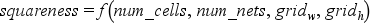
\includegraphics{./square_f.png}
            \caption{Squareness Function}
        \end{figure}

        Once we have an equation that can estimate the squareness we can plug
        in different grid dimensions and figure out one that gets us the best
        squareness. In order to figure out the formula that estimates our
        squareness we manually specified various grid dimensions for each
        benchmark and recorded the resulting squareness. This data can be found
        in the Appendix section at the end of the report. We then used the
        program Eureqa to evolve an equation that fit our data. After running
        Eureqa for 15 minutes we had an equation that fit our data with an $
        R^{2} =  0.9965 $.

        \begin{figure}[H]
            \centering
            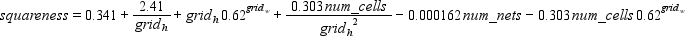
\includegraphics[width=\linewidth]{./square_eq.png}
            \caption{Squareness Equation}
        \end{figure}

        To calculate the placement grid size we start the grid as a perfect
        square by taking the square root of the number of cells. We then
        decrease the height and increase the width and check the squareness of
        this size. We continue doing this and keeping track of which size
        results in the best squareness until the height is 0.

        The table below shows the resulting squareness of the original method
        (just making a perfectly square grid) versus using the equation. We
        can see that by using the equation we achieved a much more square
        layout for all but benchmark 9. This could be a result of not having
        enough data points to fit a better curve with.

        \begin{table}[H]
            \centering
            \begin{tabular}{c|ccc|ccc|c}
                \toprule
                & \multicolumn{3}{c}{\specialcell{Without Equation}} & \multicolumn{3}{|c|}{\specialcell{With Equation}} & \\
                \textbf{Benchmark} &
                \specialcell{Grid\\Width} & \specialcell{Grid\\Height} & \specialcell{Squareness} &
                \specialcell{Grid\\Width} & \specialcell{Grid\\Height} & \specialcell{Squareness} &
                \specialcell{Percent\\Improvement} \\
                \midrule
                 1  & \phantom{0}7 & \phantom{0}7 & 0.7245 & \phantom{0}9 & \phantom{0}5 & 1.0789 &           19.66 \% \\
                 2  &           10 & \phantom{0}9 & 0.7365 &           12 & \phantom{0}8 & 0.9845 &           24.80 \% \\
                 3  &           14 &           13 & 0.6767 &           18 &           10 & 1.0914 &           23.18 \% \\
                 4  &           19 &           19 & 0.7029 &           28 &           13 & 1.2579 & \phantom{0}3.92 \% \\
                 5  &           27 &           27 & 0.6125 &           45 &           16 & 1.2060 &           18.16 \% \\
                 6  &           32 &           32 & 0.6060 &           56 &           18 & 1.1735 &           22.05 \% \\
                 7  &           23 &           22 & 0.6452 &           39 &           13 & 0.9823 &           33.71 \% \\
                 8  &           30 &           30 & 0.6306 &           50 &           18 & 1.3123 & \phantom{0}5.70 \% \\
                 9  &           29 &           28 & 0.6343 &           45 &           18 & 1.4323 &           -6.67 \% \\
                 10 &           25 &           24 & 0.6715 &           36 &           17 & 1.2772 & \phantom{0}5.13 \% \\
                \bottomrule
            \end{tabular}
            \caption{Improvement from using squareness estimate equation}
        \end{table}

        \newpage
        \subsubsection{Force Directed Placement}

        We use a force directed placement algorithm in order to reduce the
        overall complexity. Our algorithm follows the one in the book exactly
        with the exception of what happens when the target cell is locked. In
        the original algorithm you search for a vacant spot to place the seed
        cell if the target cell is locked, we expand that to also include
        unlocked spots. If we choose an unlocked spot then that cell we are
        replacing becomes the new seed cell.  We found through experimentation
        that this achieves less complex placements. The gray cells are cells
        with no connections.

        \begin{figure}[H]
            \centering
            \includegraphics[width=\linewidth, height=2in, keepaspectratio]{../benchmarks/10_placement_0_start.jpg}
            \caption{Original}
        \end{figure}
        \begin{figure}[H]
            \centering
            \includegraphics[width=\linewidth, height=2in, keepaspectratio]{../benchmarks/10_placement_1_force.jpg}
            \caption{Force Directed}
        \end{figure}

        In order to figure out the best abort limit we recorded the layout area
        for each benchmark for various limits. We found the abort limit that
        achieved the minimum area and used that minimum area to normalize the
        areas of the others as a percent increase. We found that an abort limit
        of 1 gives us the lowest average percent increase in area across all
        the benchmarks.

        \begin{figure}[H]
            \centering
            \begin{minipage}{.5\textwidth}
                \centering
                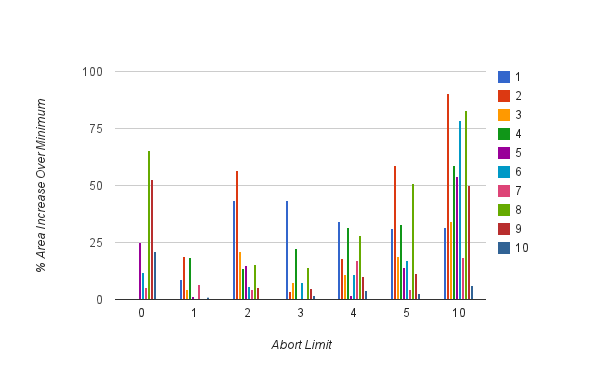
\includegraphics[width=0.98\linewidth]{./abort_limit.png}
            \end{minipage}%
            \begin{minipage}{.5\textwidth}
                \centering
                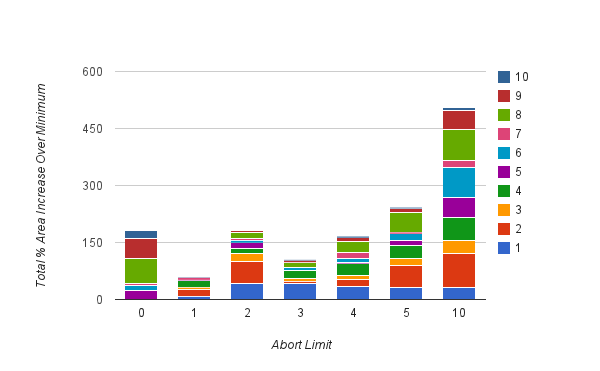
\includegraphics[width=0.98\linewidth]{./abort_limit_stacked.png}
            \end{minipage}
            \caption{Percent increase in layout area versus abort limit}
        \end{figure}

        \subsubsection{Flipping Cells}

        The force directed algorithm does not take into account the positions
        of the terminals on each cell, it assumes all connections go to the
        center of the cell. This results in a lot of connections that
        unnecessarily span vertically across a row. To fix these we simply go
        through each cell and try all possible flip orientations and see which
        one reduces the wirelength the most. This approach is not ideal as it
        does not take into consideration chains of cells that all may need to
        be flipped. An approach similar to KL where we walk down the connection
        tree trying flips and only actually flip as many as what improves
        the total wirelength would be interesting. Unfortunately we did not
        have time to explore this.

        \begin{figure}[H]
            \centering
            \includegraphics[width=\linewidth, height=4in, keepaspectratio]{../benchmarks/10_placement_1_force.jpg}
            \caption{Original}
        \end{figure}
        \begin{figure}[H]
            \centering
            \includegraphics[width=\linewidth, height=4in, keepaspectratio]{../benchmarks/10_placement_2_flip.jpg}
            \caption{Flipped}
        \end{figure}

        \subsubsection{Adding Feed-Through Cells}

        In order to channel route we cannot have connections that span rows. To
        fix this we add feed through cells (shown in light gray) in order to
        transfer the nets between rows. The process of adding feed-through cells
        starts at the bottom row. It goes through each terminal of each cell
        and detects if the terminal is in the same channel as its destination
        terminal. If it's not, it figures out if it needs to add a feed-through
        to the current row (say the terminal is at the bottom of the cell and
        it needs to connect to somewhere above it) or if it needs to add the
        feed through to the next row up (if the terminal is at the top of the
        cell but it connects to the top of the cell above it). If a feed-through
        cell is added the whole row is rescanned since we might need to
        add yet another feed through cell for the feed through we just placed.

        \begin{figure}[H]
            \centering
            \includegraphics[width=\linewidth, height=4in, keepaspectratio]{../benchmarks/10_placement_2_flip.jpg}
            \caption{Original}
        \end{figure}
        \begin{figure}[H]
            \centering
            \includegraphics[width=\linewidth, height=4in, keepaspectratio]{../benchmarks/10_placement_3_feed.jpg}
            \caption{With feed throughs}
        \end{figure}

        \subsubsection{Evening Row Lengths}

        After adding the feed-through cells the row lengths become uneven. In
        order to fix this we add all unconnected cells to a queue and then go
        through them adding them to which ever row is currently the shortest.
        Additionally we alternate placing them on either side and we also skip
        every other cell. The reason behind this is that since we just messed
        up a lot of the force directed work by removing all the unconnected
        cells we will have to re-force direct them within their rows. Spacing
        them out will allow them to more easily move around and have a higher
        chance of finding a vacant spot close to their target.

        \begin{figure}[H]
            \centering
            \includegraphics[width=\linewidth, height=4in, keepaspectratio]{../benchmarks/10_placement_3_feed.jpg}
            \caption{Original}
        \end{figure}
        \begin{figure}[H]
            \centering
            \includegraphics[width=\linewidth, height=4in, keepaspectratio]{../benchmarks/10_placement_4_feed_even.jpg}
            \caption{Even length rows}
        \end{figure}

        \subsubsection{Pulling Cells Closer}

        After evening out the row lengths we are left with a lot of space
        between connected cells. In order to fix this we run a simplified force
        directed algorithm which goes through each cell, calculates its zero
        force location on the x axis, and then finds the closest unconnected
        cell to that location and swaps its position with it.

        \begin{figure}[H]
            \centering
            \includegraphics[width=\linewidth, height=4in, keepaspectratio]{../benchmarks/10_placement_4_feed_even.jpg}
            \caption{Original}
        \end{figure}
        \begin{figure}[H]
            \centering
            \includegraphics[width=\linewidth, height=4in, keepaspectratio]{../benchmarks/10_placement_5_pull.jpg}
            \caption{Cells pulled closer}
        \end{figure}

        \newpage
        \subsubsection{Moving Feed-Through Cells}

        Sometimes, because it can not be know at the time of placement, the
        feed through cells end up on the far side of the cell as shown in the
        before picture. We make an effect to detect these and move them closer.
        We always want the feed through cell to horizontally between the two
        terminals it is connected to.

        \begin{figure}[H]
            \centering
            \begin{minipage}{.5\textwidth}
                \centering
                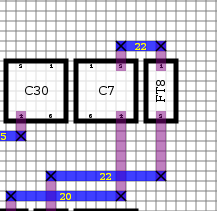
\includegraphics[width=0.98\linewidth]{./move_ft_before.png}
                \caption{Before}
            \end{minipage}%
            \begin{minipage}{.5\textwidth}
                \centering
                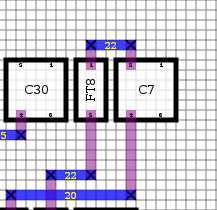
\includegraphics[width=0.98\linewidth]{./move_ft_after.png}
                \caption{After}
            \end{minipage}
        \end{figure}


\newpage
\subsection{Routing}

    \subsubsection{Assigning nets to track}

        Routing begins by first assigning each net to its own track.

        \begin{figure}[H]
            \centering
            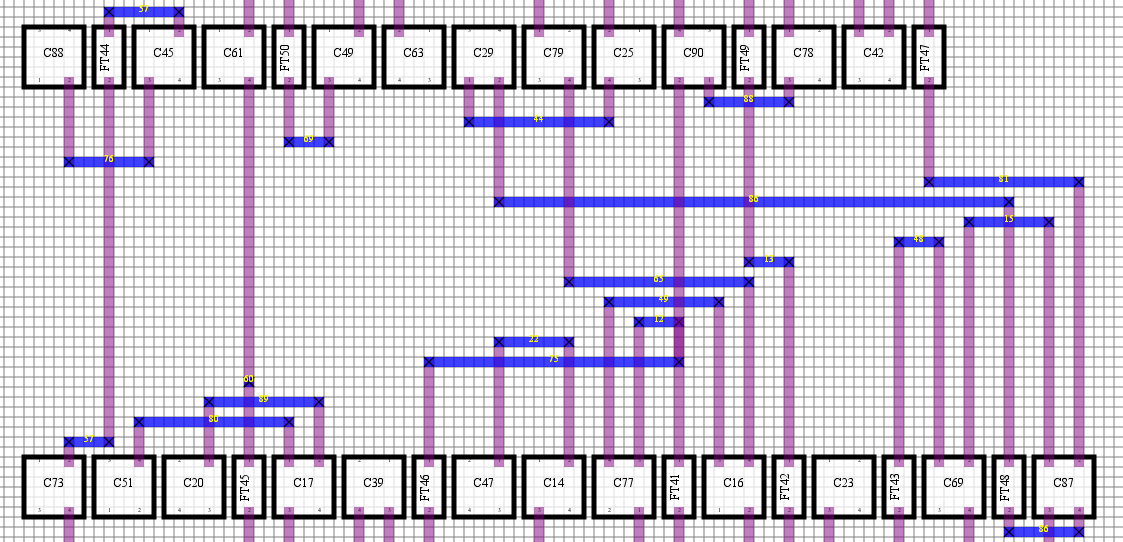
\includegraphics[width=\linewidth]{./route_0_crop.png}
            \caption{Each net has its own track}
        \end{figure}

    \subsubsection{Expand the tracks}

        Each net is checked to see if it conflicts with another net. Some
        conflict configurations can be solved by adding another track to the
        channel (expanding the channel). The solved conflict is circled in red.

        \begin{figure}[H]
            \centering
            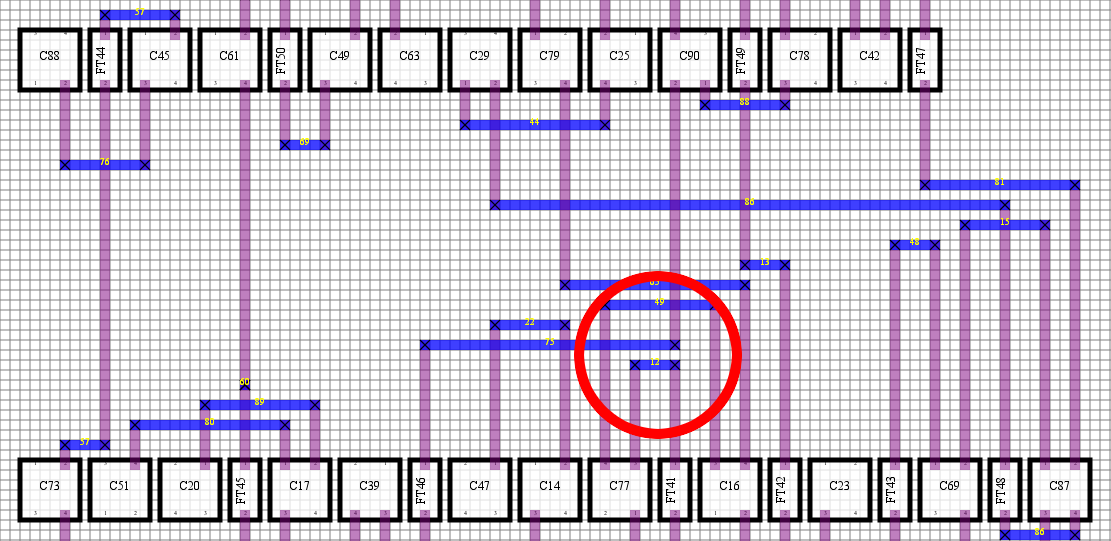
\includegraphics[width=\linewidth]{./route_1_crop.png}
            \caption{Conflict is solved by expanding the channel}
        \end{figure}

    \subsubsection{Fixing overlaps}

        Some conflicts are true overlaps that cannot be solved no matter what
        net ordering you try. The only way to solve these conflicts is to move
        the cells in the rows over. The image on the left shows an overlap
        between nets 11 and 29. The only way to solve this is to move cell C36
        over to the right, which is shown in the image on the right.

        \begin{figure}[H]
            \centering
            \begin{minipage}{.5\textwidth}
                \centering
                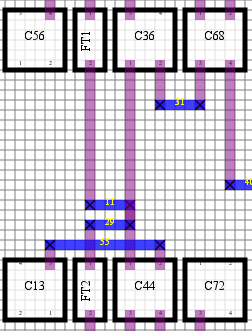
\includegraphics[width=0.75\linewidth]{./route_1_overlap.png}
                \caption{Overlapping nets}
            \end{minipage}%
            \begin{minipage}{.5\textwidth}
                \centering
                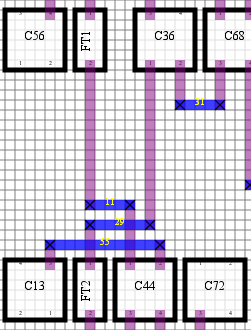
\includegraphics[width=0.75\linewidth]{./route_2_crop.png}
                \caption{Conflict is solved by moving cells over}
            \end{minipage}
        \end{figure}

    \subsubsection{Finding Vertical Nets}

        For terminals that line up directly with their destination we can use a
        purely vertical net that doesn't take up a track. The image on the left
        shows a small horizontal segment that is currently occupying a track.
        We simply mark this net as purely vertical and remove it from any
        future track related operations.

        \begin{figure}[H]
            \centering
            \begin{minipage}{.5\textwidth}
                \centering
                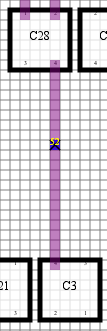
\includegraphics[height=3in]{./route_2_vertical.png}
                \caption{Vertical net taking up a track}
            \end{minipage}%
            \begin{minipage}{.5\textwidth}
                \centering
                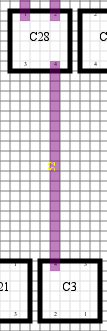
\includegraphics[height=3in]{./route_3_crop.png}
                \caption{Unnecessary horizontal segment removed}
            \end{minipage}
        \end{figure}

    \subsubsection{Pulling Nets Up}

        We next want to try to shrink the channel so the first step is to pull
        all the nets either up or down. The image below shows the result of
        pulling all the nets up and then removing tracks which not longer have
        any nets on it.

        \begin{figure}[H]
            \centering
            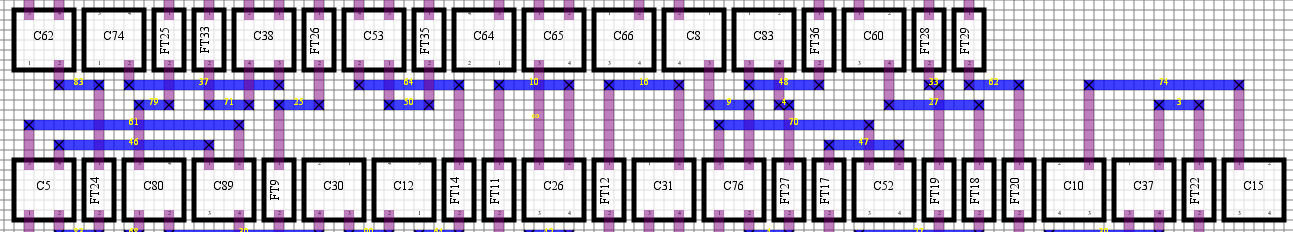
\includegraphics[width=\linewidth]{./route_4_crop.png}
            \caption{All nets pulled up and empty tracks removed}
        \end{figure}

    \subsubsection{Pulling Nets In}

        For nets whos terminals are both on the same side of the channel we
        want to bring that net back to that side (pull it in to the side the
        terminals are on). The image below shows the result of doing that.

        \begin{figure}[H]
            \centering
            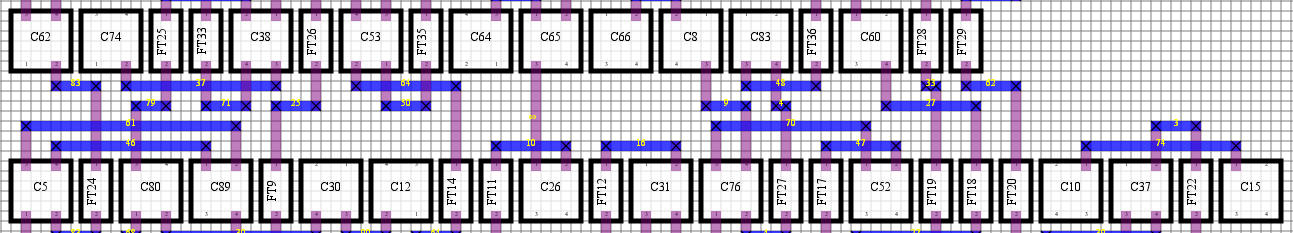
\includegraphics[width=\linewidth]{./route_5_crop.png}
            \caption{Nets pulled in closest to the cells the connect to}
        \end{figure}

        In our actual implementation we pull the cells up, then in, then down,
        then in again. This routine seems to be able to achieve fairly high
        channel density.

\newpage
\section{Usage}


\newpage
\section{Results}

    \begin{table}[H]
        \centering
        \begin{tabular}{ccccccccc}
            \toprule
            \textbf{Benchmark} &
            \specialcell{Box X} & \specialcell{Box Y} & \specialcell{Box Area} &
            \specialcell{\# FTs} & \specialcell{Wirelength} & \specialcell{\# Vias} &
            \specialcell{Execution Time} & \specialcell{Memory Usage}\\
            \midrule
            \phantom{0}1 & \phantom{00}82 & \phantom{00}76 & \phantom{000}6232 & \phantom{00}17 & \phantom{00}1093 & \phantom{0}112 & 0.009873s & \phantom{0}296 kB \\
            \phantom{0}2 & \phantom{0}127 & \phantom{0}129 & \phantom{00}16383 & \phantom{00}50 & \phantom{00}2547 & \phantom{0}270 & 0.021806s & \phantom{0}340 kB \\
            \phantom{0}3 & \phantom{0}191 & \phantom{0}175 & \phantom{00}33425 & \phantom{0}112 & \phantom{00}6114 & \phantom{0}562 & 0.044696s & \phantom{0}424 kB \\
            \phantom{0}4 & \phantom{0}317 & \phantom{0}252 & \phantom{00}79884 & \phantom{0}213 & \phantom{0}14108 & \phantom{}1126 & 0.111609s & \phantom{0}588 kB \\
            \phantom{0}5 & \phantom{0}486 & \phantom{0}403 & \phantom{0}195858 & \phantom{0}464 & \phantom{0}41469 & \phantom{}2336 & 0.384445s & \phantom{0}916 kB \\
            \phantom{0}6 & \phantom{0}602 & \phantom{0}513 & \phantom{0}308826 & \phantom{0}685 & \phantom{0}70536 & \phantom{}3322 & 0.670760s & \phantom{}1204 kB \\
            \phantom{0}7 & \phantom{}1110 & \phantom{}1130 & \phantom{}1254300 & \phantom{}1738 & \phantom{}443767 & \phantom{}5448 & 1.581445s & \phantom{}1512 kB \\
            \phantom{0}8 & \phantom{0}437 & \phantom{0}333 & \phantom{0}145521 & \phantom{0}297 & \phantom{0}22907 & \phantom{}1994 & 0.360278s & \phantom{0}912 kB \\
            \phantom{0}9 & \phantom{0}328 & \phantom{0}229 & \phantom{00}75112 & \phantom{00}69 & \phantom{00}6097 & \phantom{0}842 & 0.206668s & \phantom{0}664 kB \\
            \phantom{}10 & \phantom{0}258 & \phantom{0}202 & \phantom{00}52116 & \phantom{00}35 & \phantom{00}2881 & \phantom{0}404 & 0.157362s & \phantom{0}544 kB \\
            \bottomrule
        \end{tabular}
        \caption{Result Summary}
    \end{table}

\foreach \i in {1,...,10} {
    \newpage
    \subsection{Benchmark \i\thinspace - Placement Steps}
    \placementimage{../benchmarks/\i_placement_0_start.jpg}      {Benchmark \i\thinspace - Step 1/7 - Initial placement}
    \placementimage{../benchmarks/\i_placement_1_force.jpg}      {Benchmark \i\thinspace - Step 2/7 - Force directed placement}
    \placementimage{../benchmarks/\i_placement_2_flip.jpg}       {Benchmark \i\thinspace - Step 3/7 - Flip cells}
    \placementimage{../benchmarks/\i_placement_3_feed.jpg}       {Benchmark \i\thinspace - Step 4/7 - Add feed throughs}
    \placementimage{../benchmarks/\i_placement_4_feed_even.jpg}  {Benchmark \i\thinspace - Step 5/7 - Even out the row length}
    \placementimage{../benchmarks/\i_placement_5_pull.jpg}       {Benchmark \i\thinspace - Step 6/7 - Pull cells in the rows closer together}
    \placementimage{../benchmarks/\i_placement_6_feed_moved.jpg} {Benchmark \i\thinspace - Step 7/7 - Move feed throughs to optimal location}

    \newpage
    \subsection{Benchmark \i\thinspace - Final Routing}
    \begin{figure}[H]
        \centering
        \includegraphics[width=\linewidth]{../benchmarks/\i.jpg}
        \caption{Benchmark \i\thinspace - Final routing}
    \end{figure}

    \newpage
    \subsection{Benchmark \i\thinspace - Magic Screenshot}
    \begin{figure}[H]
        \centering
        \includegraphics[width=\linewidth]{./magic_\i.png}
        \caption{Benchmark \i\thinspace - Magic Screenshot}
    \end{figure}

    \newpage
    \subsection{Benchmark \i\thinspace - Log file}
    \lstinputlisting[caption=Benchmark \i\thinspace - Log]{../benchmarks/\i.log}
}

\newpage
\section{Performance Trends}

\newpage
\section{Appendix}

\begin{table}[H]
    \centering
    \begin{tabular}{cccccc}
        \toprule
        \textbf{Benchmark} & \textbf{Num Cells} & \textbf{Num Nets} & \textbf{Grid Width} & \textbf{Grid Height} & \textbf{Squareness}\\
        \midrule

        1  & 45   & 45   & 7  & 7  & 0.72449 \\
        2  & 90   & 90   & 10 & 9  & 0.736486 \\
        3  & 180  & 180  & 14 & 13 & 0.676724 \\
        4  & 360  & 360  & 19 & 19 & 0.702857 \\
        5  & 720  & 720  & 27 & 27 & 0.612457 \\
        6  & 1000 & 1000 & 32 & 32 & 0.605988 \\
        7  & 500  & 1000 & 23 & 22 & 0.645203 \\
        8  & 900  & 720  & 30 & 30 & 0.630648 \\
        9  & 800  & 360  & 29 & 28 & 0.634349 \\
        10 & 600  & 180  & 25 & 24 & 0.67148 \\
        \midrule

        1  & 45   & 45   & 8  & 6  & 0.820225 \\
        2  & 90   & 90   & 27 & 8  & 0.984496 \\
        3  & 180  & 180  & 12 & 12 & 0.755981 \\
        4  & 360  & 360  & 15 & 18 & 0.740413 \\
        5  & 720  & 720  & 20 & 26 & 0.595577 \\
        6  & 1000 & 1000 & 28 & 31 & 0.561298 \\
        7  & 500  & 1000 & 33 & 21 & 0.614935 \\
        8  & 900  & 720  & 24 & 29 & 0.637652 \\
        9  & 800  & 360  & 32 & 27 & 0.685294 \\
        10 & 600  & 180  & 30 & 23 & 0.75 \\
        \midrule

        1  & 45   & 45   & 9  & 5  & 1.078947 \\
        2  & 90   & 90   & 13 & 7  & 1.20339 \\
        3  & 180  & 180  & 17 & 11 & 0.921875 \\
        4  & 360  & 360  & 22 & 17 & 0.833333 \\
        5  & 720  & 720  & 29 & 25 & 0.681979 \\
        6  & 1000 & 1000 & 34 & 30 & 0.583232 \\
        7  & 500  & 1000 & 25 & 20 & 0.646465 \\
        8  & 900  & 720  & 33 & 28 & 0.672032 \\
        9  & 800  & 360  & 31 & 26 & 0.731629 \\
        10 & 600  & 180  & 28 & 22 & 0.773946 \\
        \midrule

        1  & 45   & 45   & 12 & 4  & 1.779661 \\
        2  & 90   & 90   & 15 & 6  & 1.623762 \\
        3  & 180  & 180  & 18 & 10 & 1.091429 \\
        4  & 360  & 360  & 23 & 16 & 0.84127 \\
        5  & 720  & 720  & 30 & 24 & 0.742911 \\
        6  & 1000 & 1000 & 35 & 29 & 0.624372 \\
        7  & 500  & 1000 & 27 & 19 & 0.692828 \\
        8  & 900  & 720  & 34 & 27 & 0.711864 \\
        9  & 800  & 360  & 32 & 25 & 0.790323 \\
        10 & 600  & 180  & 29 & 21 & 0.869748 \\
        \midrule

        1  & 45   & 45   & 15 & 3  & 2.923077 \\
        2  & 90   & 90   & 18 & 5  & 1.864583 \\
        3  & 180  & 180  & 20 & 9  & 1.322368 \\
        4  & 360  & 360  & 24 & 15 & 0.920382 \\
        5  & 720  & 720  & 32 & 23 & 0.75098 \\
        6  & 1000 & 1000 & 36 & 28 & 0.699068 \\
        7  & 500  & 1000 & 28 & 18 & 0.715323 \\
        8  & 900  & 720  & 35 & 26 & 0.694501 \\
        9  & 800  & 360  & 34 & 24 & 0.810289 \\
        10 & 600  & 180  & 30 & 20 & 0.991111 \\
        \midrule

        1  & 45   & 45   & 23 & 2  & 4.945946 \\
        2  & 90   & 90   & 23 & 4  & 2.626667 \\
        3  & 180  & 180  & 23 & 8  & 1.391608 \\
        4  & 360  & 360  & 26 & 14 & 0.986532 \\
        5  & 720  & 720  & 33 & 22 & 0.848671 \\
        6  & 1000 & 1000 & 38 & 27 & 0.674667 \\
        7  & 500  & 1000 & 30 & 17 & 0.763196 \\
        8  & 900  & 720  & 36 & 25 & 0.832599 \\
        9  & 800  & 360  & 35 & 23 & 0.883333 \\
        10 & 600  & 180  & 32 & 19 & 1.074074 \\

        \bottomrule
    \end{tabular}
    \caption{Squareness Trial Data}
\end{table}


\end{document}
